\begin{figure*}
\centering
\begin{subfigure}{0.8\textwidth}
\centering
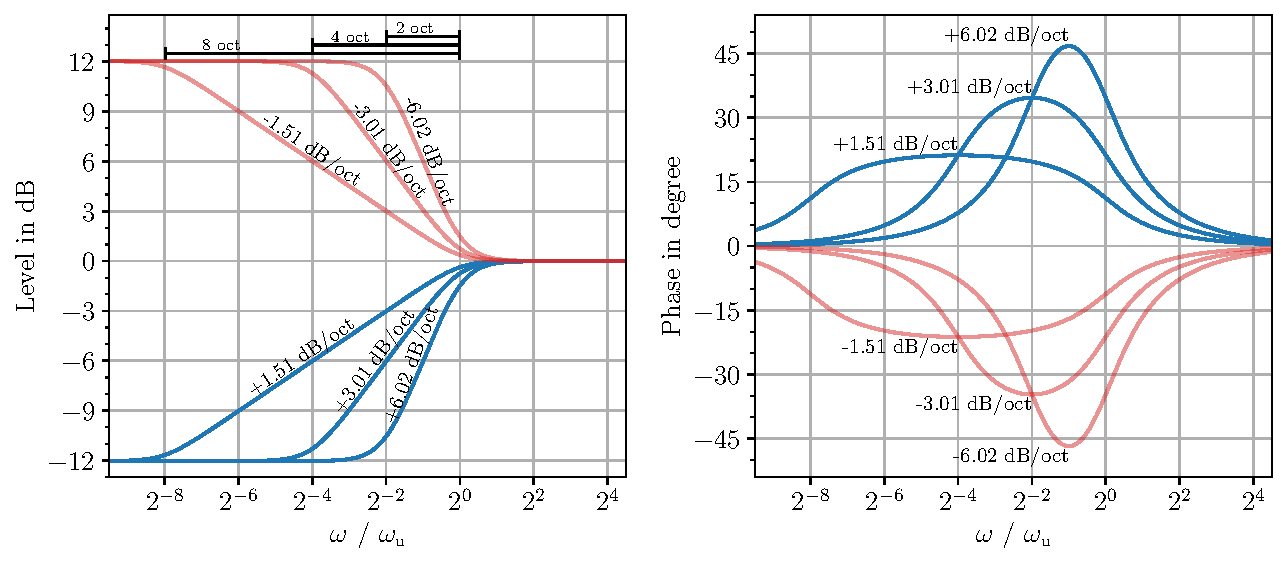
\includegraphics[width=\textwidth]{../graphics/low-shelving-filter-varying-slope.pdf}
\caption{Fixed shelving level $G=\pm 20 \lg (4) \approx \pm 12$ dB.
Varied slope $\chi$ in
dB/oct with resulting bandwidth $\beta$ in octaves or vice versa.}
\label{fig:low-shelving-filter-varying-slope}
\end{subfigure}
\\
\begin{subfigure}{0.8\textwidth}
\centering
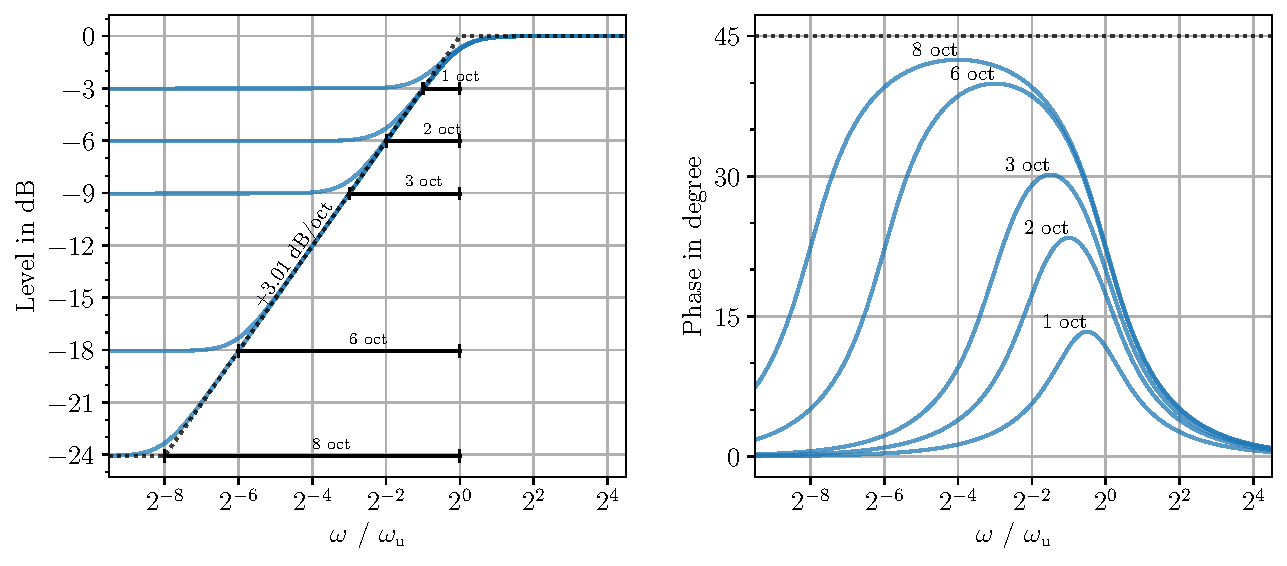
\includegraphics[width=\textwidth]{../graphics/low-shelving-filter-varying-bandwidth.pdf}
\caption{Fixed slope $\chi = 10\lg(2)\approx + 3.01$ dB/oct. Varied bandwidth
$\beta$ in octaves, resulting shelving level $G$ in dB or vice versa.}
\label{fig:low-shelving-filter-varying-bandwidth}
\end{subfigure}
\\
\begin{subfigure}{0.8\textwidth}
\centering
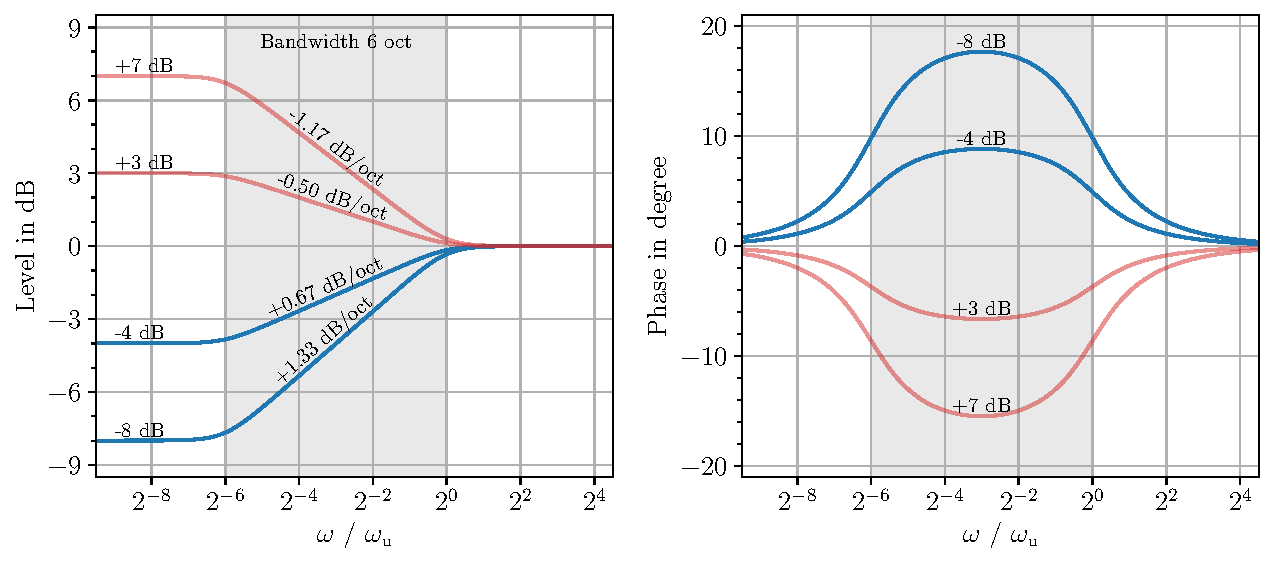
\includegraphics[width=\textwidth]{../graphics/low-shelving-filter-varying-gain.pdf}
\caption{Fixed bandwidth $\beta=6$ octaves. Varied shelving level $G$ in dB,
resulting slope $\chi$ in dB/octave or vice versa.}
\label{fig:low-shelving-filter-varying-gain}
\end{subfigure}
%
\caption{Shelving filter cascade frequency responses.
Two of the three design parameters $\chi$, $\beta$ and $G$
can be freely chosen, determining the third one. Depending on the target
application one of the three setup strategies might be preferable.}
\label{fig:shelving_filter_setup_cases}
\end{figure*}
